\documentclass[a4paper,oneside,svgnames,draft]{amsart}

\usepackage[T1]{fontenc}
\usepackage[utf8]{inputenc}

\usepackage{xcolor}
\usepackage[colorlinks=true,citecolor=Green]{hyperref}
\usepackage{amsrefs}
\usepackage{tikz}
\usepackage[noabbrev]{cleveref} 

% Theorems
\theoremstyle{plain}
\newtheorem{theorem}{Theorem}[section]
\newtheorem{proposition}[theorem]{Proposition}
\newtheorem{lemma}[theorem]{Lemma}

\theoremstyle{definition}
\newtheorem{definition}[theorem]{Definition}

\title{Research Statement}
\author{Adam Klepáč}
\date{\today}

\begin{document}
 \maketitle
 \begin{abstract}
  Following the construction of $d$-representation-finite algebras
  in~\cite{iyama} and the description of the correspondence between certain
  types of cluster algebras and triangulations of bordered surfaces with marked
  points in~\cite{fst}, links have appeared connecting $d$-representation finite
  algebras to higher dimensional variants of said surface. One such link was
  discovered in~\cite{ot} between higher Auslander algebras of the path algebra
  of linearly oriented Dynkin quiver $A_n$ and cyclic polytopes. I wish to
  further study such kinds of connections, starting with the establishment of a
  similar type of link for path algebras of quivers of type $D_n$ which, in the
  low-dimensional case, correspond to once punctured polygons; then, with a
  touch of expectation and naïvety, broadening it to include (special types of)
  cluster algebras not necessarily representation-finite.
 \end{abstract}

 \section{Introduction}
 \label{sec:introduction}

 This text serves primarily as an overview of relevant concepts regarding
 cluster algebras, bordered surfaces with marked points, higher dimensional
 cluster categories and $d$-representation-finite algebras interwoven with ideas
 of possible generalizations and caveats tied to such endeavour. So far, I have
 only scratched the surface of this topic, hence very few original results are
 present.

 % TODO links
 In Section 2, I give a summary of the theory of bordered surfaces with marked
 points. Section 3 is dedicated to (normalized skew-symmetrizable) cluster
 algebras and their connection to bordered surfaces with marked points is drawn.
 Sections 4 and 5 define $d$-representation-finite algebras and higher cluster
 categories, respectively. Section 6 summarizes relevant results
 from~\cite{ot}, regarding a higher-dimensional kind of connection described in
 Section 3. Finally, Section 7 is riddled with (splinters of) steps towards
 generalizations of the content of Section 6.

 \section{Bordered Surfaces with Marked Points}
 \label{sec:bordered-surfaces-with-marked-points}

 This section is a brief summary of~\cite{fst}, Section 2.
 \begin{definition}[Bordered surface with marked points]
  \label{def:marked-surface}
  Let $\mathbf{S}$ be a connected oriented $2$-dimensional Riemann surface with
  boundary. We fix a finite set $\mathbf{M}$ of \emph{marked points} in the
  closure of $\mathbf{S}$. Marked points lying in the interior of $\mathbf{S}$
  are called \emph{punctures}. The pair $(\mathbf{S},\mathbf{M})$ is called a
  \emph{bordered surface with marked points} if the following additional
  technical conditions are satisfied.
  \begin{itemize}
   \item The set $\mathbf{M}$ is non-empty.
   \item The pair $(\mathbf{S}, \mathbf{M})$ is not
   \begin{itemize}
    \item a sphere with one or two punctures;
    \item a monogon with zero or one puncture;
    \item a digon without punctures;
    \item a triangle without punctures.
   \end{itemize}
  \end{itemize}
  Here, the term $n$-gon denotes a disk with $n$ marked points on its boundary.
  Moreover, sphere with three punctures is also often excluded.
 \end{definition}

 \begin{definition}[Arc]
  \label{def:arc}
  An arc $\gamma$ in a bordered surface with marked points
  $(\mathbf{S},\mathbf{M})$ is a curve in $\mathbf{S}$ such that
  \begin{itemize}
   \item its endpoints are marked points;
   \item $\gamma$ does not intersect itself, except that its endpoints may
    coincide;
   \item except for its endpoints, $\gamma$ is disjoint from $\mathbf{M}$ and
    from the boundary of $\mathbf{S}$;
   \item $\gamma$ is not contractible into $\mathbf{M}$ or into the boundary of
    $\mathbf{S}$.
  \end{itemize}
 \end{definition}

 We are interested in triangulations of $(\mathbf{S},\mathbf{M})$. Vaguely
 speaking, triangulation is a division of $\mathbf{S}$ into `triangles' by a
 series of `cuts'. Here, `triangles' are either disks with three marked points
 on their boundaries or, so-called \emph{self-folded} triangles, once-punctured
 monogons with an arc connecting the unique marked point to the unique puncture.
 See \cref{fig:self-folded-triangle}.
 \begin{figure}[ht]
  \centering
  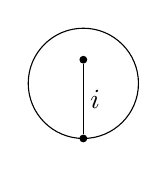
\begin{tikzpicture}
   \node[circle,fill,inner sep=1pt] (a) at (0,0) {};
   \node[circle,fill,inner sep=1pt] (b) at (0,1) {};

   \draw (a) to node[midway,xshift=1.5mm] {$i$} (b);
   \draw (0,0.7) circle[radius=0.7];
  \end{tikzpicture}

  \caption{A self-folded triangle.}
  \label{fig:self-folded-triangle}
 \end{figure}

 \begin{definition}[Isotopy]
  \label{def:isotopy}
  Let $\gamma_1,\gamma_2$ be two arcs in $(\mathbf{S},\mathbf{M})$. An
  \emph{isotopy} between $\gamma_1$ and $\gamma_2$ is a homotopy $H$ between
  $\gamma_1$ and $\gamma_2$ such that $H(x,t)$ is an embedding for each fixed
  $t \in [0,1]$. Isotopy is an equivalence relation on the set of all arcs in
  $(\mathbf{S},\mathbf{M})$.
 \end{definition}
 In the following text, each arc in $(\mathbf{S},\mathbf{M})$ is considered up
 to isotopy.

 \begin{definition}[Compatibility of arcs]
  \label{def:compatibility-of-arcs}
  Two arcs in $(\mathbf{S},\mathbf{M})$ are called \emph{compatible} if they (up
  to isotopy) do not intersect each other in the interior of $\mathbf{S}$.
 \end{definition}

 \begin{proposition}
  \label{prop:triangulation-up-to-isotopy}
  Any collection of pairwise compatible arcs can be realized by curves in their
  respective isotopy classes which do not intersect in the interior of
  $\mathbf{S}$.
 \end{proposition}

 \begin{definition}[Ideal triangulation]
  \label{def:ideal-triangulation}
  A maximal collection of pairwise compatible arcs is called an \emph{ideal
  triangulation}. In fact, \cref{def:marked-surface} excludes all cases where
  $(\mathbf{S},\mathbf{M})$ cannot be triangulated. The arcs of an ideal
  triangulation cut $\mathbf{S}$ into \emph{ideal triangles}. The three sides of
  an ideal triangle need not be distinct, leading to self-folded triangle, and
  two triangles can share more than one side.
 \end{definition}

 \bibliography{refs.bib}
\end{document}
